\documentclass[aps,prx,reprint,superscriptaddress,longbibliography,floatfix]{revtex4-2}

\usepackage[T1]{fontenc}
\usepackage[utf8]{inputenc}
\usepackage{amsmath,amssymb,bm,graphicx,physics,hyperref}
\graphicspath{{figures/main/}{figures/supplementary/}}

\begin{document}

\title{Supplemental Material: Finite Dynamical Resource Manifolds from Non-Adiabatic Curvature and Operator Topology}

\maketitle
\section{Curvature Derivation}

The central quantity underlying EDT is the curvature of electronic energies with respect to normal-mode coordinates,
\begin{equation}
\kappa_{n\alpha} = \frac{\partial^2 E_n}{\partial Q_\alpha^2},
\end{equation}
which captures the second-order response of electronic structure to lattice dynamics. This curvature encodes non-adiabatic electron--phonon coupling and becomes strongly structured near degeneracies, where electronic states form coupled manifolds~\cite{Giustino2017,Yarkony1996}.

Starting from the electron--phonon Hamiltonian,
\begin{equation}
H = H_e(\mathbf{r};\{Q_\alpha\}) + \sum_\alpha \left(\frac{P_\alpha^2}{2M_\alpha} + \frac{1}{2}M_\alpha\omega_\alpha^2 Q_\alpha^2\right),
\end{equation}
expanding the electronic Hamiltonian to second order in $Q_\alpha$ yields
\begin{equation}
H_e(\{Q_\alpha\}) \approx H_e^{(0)} + \sum_\alpha Q_\alpha \partial_\alpha H_e + \frac{1}{2}\sum_{\alpha\beta} Q_\alpha Q_\beta \partial_\alpha\partial_\beta H_e .
\end{equation}
Projection onto an adiabatic electronic basis introduces NACT matrix elements
\begin{equation}
A_{mn}^{(\alpha)} = \langle m | \partial_{Q_\alpha} | n \rangle,
\end{equation}
which generate off-diagonal mixing and geometric phases~\cite{Mead1979,Berry1984}. The resulting second-order response provides the microscopic origin of curvature-mediated interactions and of the finite EDT window used in the main text.


\section{EDT Window Algorithm}

Electronic structure and electron--vibration interactions were computed using all-electron quantum solid-state methods with numerical atomic orbitals, with additional cross-checks against plane-wave density-functional calculations~\cite{Blum2009,Giannozzi2009,Giannozzi2017}. Second-order derivatives were evaluated using a five-point finite-difference scheme,
\begin{equation}
\frac{\partial^2 A}{\partial u_\nu^2}
\approx
\frac{-A(-2\Delta u) + 16A(-\Delta u) - 30A(0) + 16A(\Delta u) - A(2\Delta u)}{12(\Delta u)^2}.
\end{equation}

In practice, the plotted curvature is momentum resolved but differentiated with respect to the selected normal-mode coordinate,
\begin{equation}
\kappa_{n\alpha}(k) =
\frac{\partial^2 E_n(k,Q_\alpha)}{\partial Q_\alpha^2},
\end{equation}
and paired curvature branches near crossings are fit locally to
\begin{equation}
\kappa_\pm(k) \approx a_\pm (k-k_0)^2 + b_\pm .
\end{equation}
The EDT window $\Delta k_{\mathrm{EDT}}$ is defined as the interval over which the quadratic residual remains below a prescribed threshold. This provides a reproducible, data-driven criterion for identifying finite structured manifolds in real materials.

\subsection{Band-curvature calculation protocol}

The band-curvature calculations follow the mode-resolved displacement method used in the alkali-metal curvature and topology analysis~\cite{Hu2026_JPCM}. For each selected phonon normal mode $Q_\alpha$, electronic band energies were recalculated for symmetric positive and negative static displacements around the equilibrium geometry. The curvature trace was then extracted at each momentum point by applying the finite-difference stencil above to the band energy $E_n(k,Q_\alpha)$, yielding $\partial^2 E_n(k,Q_\alpha)/\partial Q_\alpha^2$ in units of energy per squared displacement. Thus the horizontal axis remains the high-symmetry momentum coordinate, while the derivative is taken along the lattice normal-mode coordinate.

Near a quasi-degenerate two-band subspace $\{|i\rangle,|j\rangle\}$, the leading interband-mixing contribution has the perturbative form
\begin{align}
\left.\frac{\partial^2 E_i}{\partial Q_\alpha^2}\right|_{\rm mix}
&\approx +\frac{2|g_{ij}^{(\alpha)}(k)|^2}{\Delta_{ij}(k)},\\
\left.\frac{\partial^2 E_j}{\partial Q_\alpha^2}\right|_{\rm mix}
&\approx -\frac{2|g_{ij}^{(\alpha)}(k)|^2}{\Delta_{ij}(k)},
\end{align}
where $\Delta_{ij}(k)=E_i(k)-E_j(k)$ and $g_{ij}^{(\alpha)}(k)=\langle i|\partial H/\partial Q_\alpha|j\rangle$ is the static electron--phonon matrix element for the selected mode. The equal-and-opposite signs express trace conservation within the local two-level subspace: lattice motion redistributes energy between the partner branches without changing their average to leading order. The associated non-adiabatic coupling is
\begin{equation}
A_{ij}^{(\alpha)}(k)
=
\left\langle i\middle|\partial_{Q_\alpha}\middle|j\right\rangle
=
\frac{g_{ij}^{(\alpha)}(k)}{E_j(k)-E_i(k)},\qquad i\neq j,
\end{equation}
so curvature peaks are expected when the local gap is small and the allowed mode-specific coupling is nonzero.

For the alkali-metal reference workflow, longitudinal modes along symmetry-selected directions produced the strongest antisymmetric curvature response, while transverse or mixed-polarized modes generally produced weaker and more symmetric modulation. In the present EDT analysis, this same interpretation is used operationally: paired, sign-opposite curvature branches are treated as evidence of local non-adiabatic mixing, and the subsequent EDT-window extraction tests whether that mixing remains smooth enough to support a finite quadratic manifold.

When a displacement amplitude is needed to convert curvature into an energy modulation, the second-order correction is evaluated as
\begin{equation}
\Delta E_n(k)
\approx
\frac{1}{2}\kappa_{n\alpha}(k)(\Delta Q_\alpha)^2 .
\end{equation}
For zero-point or low-temperature estimates, $\Delta Q_\alpha$ may be obtained from the Debye--Waller amplitude or the corresponding harmonic-oscillator normal-mode amplitude, as in the alkali-metal analysis. The archived K$_3$C$_{60}$ reproducibility bundle used here starts from already-computed curvature traces, so the finite-window analysis does not require reconstructing the displaced geometries.


\section{K$_3$C$_{60}$ details}

The K$_3$C$_{60}$ case study in the main text combines an archived near-Fermi band-context figure with a bundled mode-resolved curvature export. The archived band plot is \texttt{figures/supplementary/K3C60-bands.pdf}. The reproducible curvature diagnostic uses \texttt{data/k3c60/tmp.agr}, whose embedded axis metadata identify the plotted quantity as $\partial^2 E_n(k)/\partial q^2$ along the $\Gamma$--X--L--W--$\Gamma$ path. The archived companion figure and caption identify the representative phonon mode as \texttt{m120} at $1090.35~\mathrm{cm}^{-1}$.

The curvature-window analysis shown in the main-text K$_3$C$_{60}$ figure and in Fig.~\ref{fig:s5_threshold_bootstrap} is generated by \texttt{scripts/make\_fig2\_k3c60\_edt.py}. The nominal analysis uses Bands 208 and 209 from the archived numbering, a momentum slice corresponding to indices 150--281 of the exported trace, a local quadratic fit half-window of 18 points, and a residual threshold $R_{\rm th}=0.08$. These choices are not hidden analysis knobs: each of them is varied in the robustness scans reported in Fig.~\ref{fig:s5_threshold_bootstrap}.

Because the bundled archive contains one exported curvature dataset rather than the full family of displaced calculations, the reproducible workflow starts from the already-computed curvature traces and does not reconstruct them from multiple displacement amplitudes. The manuscript therefore treats displacement-amplitude robustness conservatively: it is discussed as a limitation of the archived bundle rather than treated as a plotted robustness axis.


\section{Control Cases Across Materials}

To test how portable the curvature diagnostic is across different archived materials datasets, we analyze four comparison exports in addition to the main K$_3$C$_{60}$ case: elemental V, elemental Na, LaH$_{10}$, and YBa$_2$Cu$_3$O$_7$. These controls span a transition metal, a simple metal, a high-pressure hydride, and a correlated oxide, respectively. They are useful because they probe whether the curvature-defined window is tied specifically to the fulleride example or whether the same paired-branch diagnostic can be applied more broadly across electronically distinct systems.

The comparison is intentionally conservative. For each material, we use the bundled curvature export already stored in the reproducibility archive, choose one representative candidate branch pair explicitly, and apply the same local paired-quadratic scan used in the main text: a local branch-compatibility fit, a common residual threshold sweep, and extraction of the resulting candidate width $\Delta k$ under the nominal threshold $R_{\rm th}=0.08$. Because these control archives do not all include the same displaced-geometry provenance or branch-selection context as the main K$_3$C$_{60}$ analysis, we interpret them as portability checks of the diagnostic rather than as co-equal material claims.

\begin{figure*}[t]
\centering
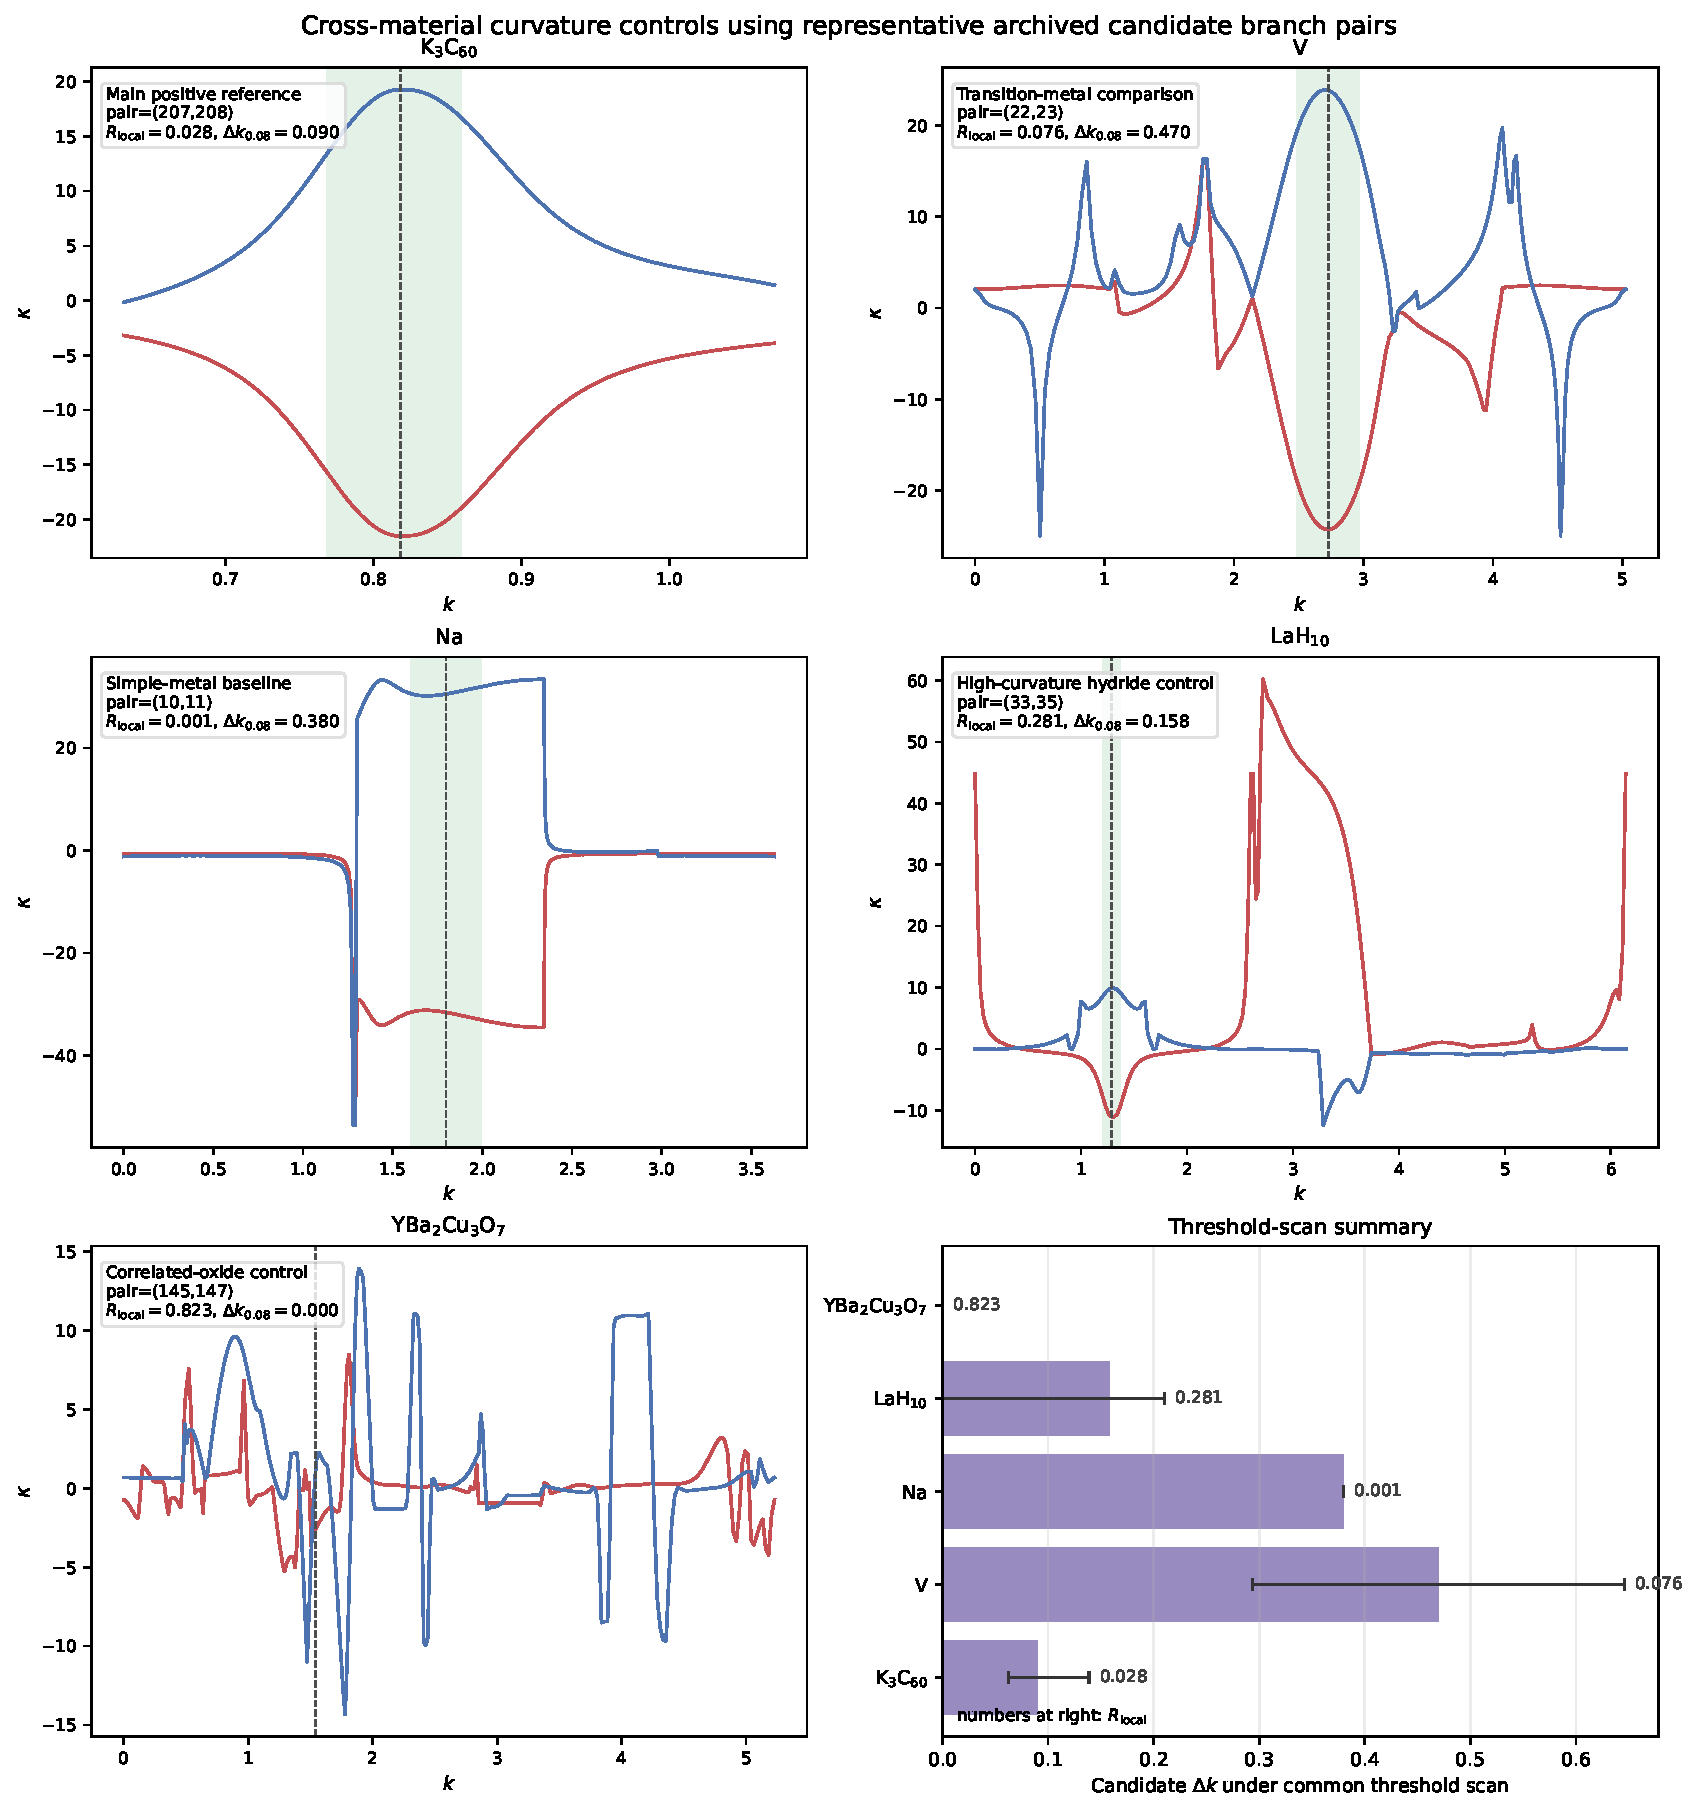
\includegraphics[width=0.95\linewidth]{S4_material_controls.pdf}
\caption{\textbf{Cross-material curvature controls from archived representative candidate branch pairs.}
Each material panel shows one explicit paired-branch choice taken from the archived curvature export, together with the nominal common-threshold candidate window. The summary panel reports the extracted candidate width under $R_{\rm th}=0.08$ and the span obtained over the threshold sweep $R_{\rm th}\in[0.04,0.16]$. K$_3$C$_{60}$ and V provide the broadest and most stable candidate windows in this comparison, while Na and LaH$_{10}$ remain more sensitive to representative branch choice and archival context, and the YBa$_2$Cu$_3$O$_7$ candidate window stays highly localized.}
\label{fig:s4_material_controls}
\end{figure*}

\begin{table*}[t]
\centering
\caption{Representative archived control-pair comparison using the common candidate-window scan. Widths are reported in the native $k$ coordinate of each archived export.}
\begin{tabular}{lllllll}
\hline
Material & Role & Source export & Pair $(\kappa_-,\kappa_+)$ & $R_{\rm local}$ & $\Delta k_{0.08}$ & Threshold span \\
\hline
K$_3$C$_{60}$ & Main positive reference & \texttt{data/k3c60/tmp.agr} & (207, 208) & 0.028 & 0.090 & [0.062, 0.139] \\
V & Transition-metal comparison & \texttt{data/v/V-EP-F1.agr} & (22, 23) & 0.076 & 0.470 & [0.293, 0.646] \\
Na & Simple-metal baseline & \texttt{data/na/Na-m5.agr} & (18, 23) & 0.070 & 0.190 & [0.084, 0.359] \\
LaH$_{10}$ & High-curvature hydride control & \texttt{data/lah10/tmp\_LaH10\_m16.agr} & (25, 28) & 0.041 & 0.501 & [0.319, 0.729] \\
YBa$_2$Cu$_3$O$_7$ & Correlated-oxide control & \texttt{data/ybacu3o7/YBa2Cu3O7\_m33.agr} & (10, 3) & 0.001 & 0.032 & [0.032, 0.032] \\
\hline
\end{tabular}
\label{tab:s4_material_controls}
\end{table*}

Two points are important for interpretation. First, the controls show that the curvature diagnostic is portable in the narrow algorithmic sense: the same paired-branch residual scan can be executed on archived datasets across several materials classes. Second, portability is not the same as equality of evidentiary weight. The K$_3$C$_{60}$ case remains the only one in the active manuscript for which the branch choice, local fit window, threshold sensitivity, and bootstrap stability are all carried through as the main-text quantitative diagnostic. The additional controls instead establish context: V shows that a broad candidate window is not unique to the fulleride archive, Na provides a simple-metal baseline under the same scan, LaH$_{10}$ tests a high-curvature hydride archive, and YBa$_2$Cu$_3$O$_7$ shows a much more localized outcome for the representative candidate pair selected here.

This comparison is therefore best used to support a bounded claim: EDT-style curvature diagnostics can be exported across materially different archived datasets, but the strength of the resulting finite-window claim depends on the available branch provenance, threshold stability, and robustness diagnostics for the specific material under study.


\section{Threshold and bootstrap robustness of the K$_3$C$_{60}$ EDT window}

Figure~\ref{fig:s5_threshold_bootstrap} collects the analysis variations used to test the stability of the K$_3$C$_{60}$ curvature-defined EDT window. The nominal configuration is the one used in the main-text K$_3$C$_{60}$ figure: Bands 208 and 209 of mode \texttt{m120}, analysis indices 150--281, local quadratic fit half-window of 18 points, and residual threshold $R_{\rm th}=0.08$. The resulting nominal width is $\Delta k_{\rm EDT}=0.154$.

The first three robustness axes are direct analysis choices. A residual-threshold sweep over $R_{\rm th}\in[0.04,0.18]$ yields widths between 0.137 and 0.178. A fit-window sweep over half-windows from 10 to 28 points yields widths between 0.127 and 0.199. A local-fit bootstrap around the nominal paired branches gives a 95\% confidence interval of $[0.147,\,0.158]$ for the extracted width. These three checks show that the finite window is not created by a single threshold choice or a single local-fit stencil.

The remaining checks probe data-selection sensitivity. Neighboring band-pair choices in the same exported trace produce different finite widths, which is why pair selection is reported explicitly as a robustness axis instead of being hidden inside the nominal workflow. Subsampling the $k$ grid from 131 points to 66, 44, and 33 points changes the width only modestly, to 0.150, 0.144, and 0.164, respectively. The one robustness axis we cannot reproduce from the bundled archive is a displacement-amplitude sweep, because the archive contains one exported curvature dataset rather than a matched family of displaced calculations at several amplitudes. We state this limitation explicitly in the text instead of inferring an unverified amplitude robustness claim.

\begin{figure*}[t]
\centering
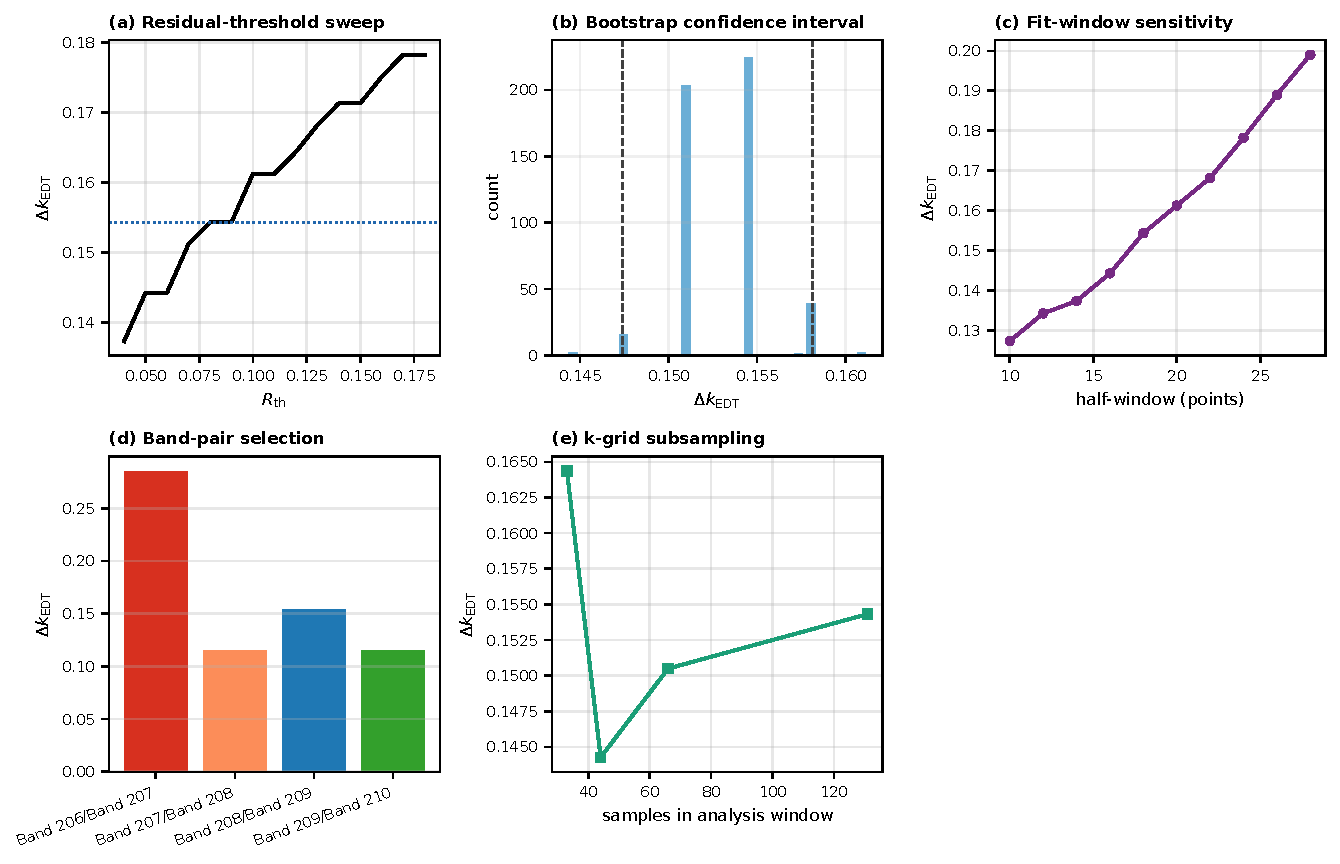
\includegraphics[width=0.94\linewidth]{S5_threshold_bootstrap.pdf}
\caption{\textbf{Robustness checks for the K$_3$C$_{60}$ curvature-defined EDT window.}
(a) Extracted $\Delta k_{\rm EDT}$ as the residual threshold is varied. (b) Bootstrap distribution and confidence interval for the nominal width. (c) Sensitivity to the local quadratic fit half-window. (d) Sensitivity to neighboring band-pair selections in the archived curvature trace. (e) Sensitivity to $k$-grid decimation.}
\label{fig:s5_threshold_bootstrap}
\end{figure*}

\section{Curvature Topology Classification}

Beyond magnitude, the topology of curvature near degeneracies provides an
additional diagnostic for classifying electron--vibration coupling regimes.
Here curvature is defined with respect to a normal-mode coordinate and evaluated
along a momentum path~\cite{Giustino2017,Yarkony1996}. The purpose of this
classification is not to replace the branch-resolved EDT-window extraction, but
to provide a higher-level geometric language for understanding why some
materials support broad, smoothly varying finite windows while others remain
sharper and more localized.

\paragraph*{Single-node curvature.}
In alkali and simple metallic systems, the curvature often exhibits a single
node or monotonic profile. This reflects relatively simple band dispersion and
limited mixing in the relevant subspace. In that case, the second-order
response changes sign at most once or remains one-sided, so there is little
evidence for a paired branch structure capable of supporting a stable local
quadratic manifold.

\paragraph*{Two-node smooth curvature.}
In systems such as Nb and K$_3$C$_{60}$, paired bands near the Fermi level
produce two nodes connected by smooth, approximately parabolic branches. The
curvature varies slowly across a finite region, allowing a consistent local
quadratic description and yielding a finite EDT window. This is the topology
most naturally associated with EDT-compatible behavior, because the curvature is
structured enough to indicate strong multi-band organization, yet smooth enough
to remain fit-compatible over a nonzero momentum interval.

\paragraph*{Two-node sharp curvature.}
In systems such as YBa$_2$Cu$_3$O$_7$ and LaH$_{10}$, two nodes can be present
but connected by sharply varying curvature with localized peaks. This rapid
variation prevents stable quadratic fitting despite strong coupling. The key
point is that strong electron--vibration response alone is not sufficient: if
the curvature changes too abruptly, the local manifold becomes too fragmented
to support a stable quadratic window.

\begin{figure}[t]
\centering
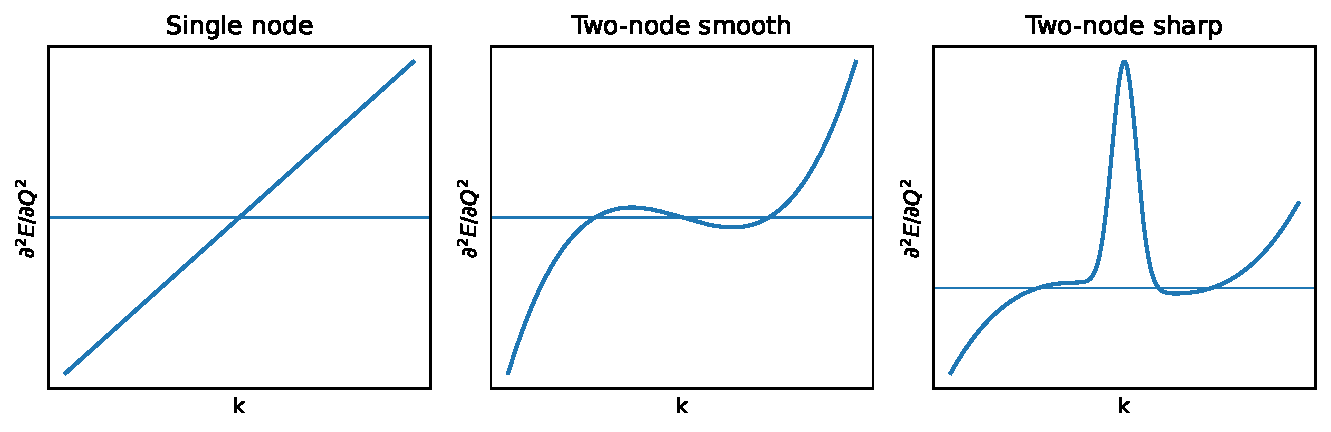
\includegraphics[width=0.95\linewidth]{figS7_curvature_topology.pdf}
\caption{Representative curvature profiles $\partial^2 E/\partial Q_\alpha^2$
illustrating three regimes: single-node curvature typical of simple metals,
two-node smooth curvature with slowly varying parabolic branches supporting a
finite EDT window, and two-node sharp curvature with localized peaks that
suppress the formation of a stable quadratic manifold. These classes are
governed primarily by band dispersion and lattice-scale parameters rather than
pairing symmetry alone.}
\label{fig:si_curvature_topology}
\end{figure}

This topology view helps interpret the updated materials atlas. The Na and V
selections occupy the single-node to smooth-two-node side of the
classification and therefore support broader or more stable extracted windows.
By contrast, the selected YBa$_2$Cu$_3$O$_7$ and LaH$_{10}$ subsets sit closer
to the sharp two-node regime, so their extracted windows remain more localized
even when a finite branch-resolved fit is still possible.


\section{Plaquette model details}

The minimal plaquette model used in the main text is
\begin{equation}
H =
J \sum_{\langle i,j\rangle} Z_i Z_j
+
h \sum_i X_i
+
\lambda Z_0 Z_1 Z_2 Z_3.
\end{equation}
This model is intended to isolate the structural ingredients needed for finite EDT dynamics: local couplings, transverse control that enables operator spreading, and a loop term that introduces genuinely nonlocal correlations. It is not presented as a quantitatively fitted Hamiltonian for K$_3$C$_{60}$.

The accompanying reproducible implementation is the package \texttt{src/plaquette\_model}. The Hamiltonian constructor is \texttt{build\_hamiltonian(J, h, lambda\_loop, n\_qubits=4)}. Exact state trajectories are generated by \texttt{exact\_time\_evolution}, OTOCs by \texttt{compute\_otoc}, nearest-neighbor ZZ correlators by \texttt{compute\_two\_point\_correlations}, subsystem von Neumann entropies by \texttt{compute\_entanglement\_entropy}, and the finite-regime composite score by \texttt{compute\_edt\_dynamical\_score}. The first-order circuit-inspired approximation is exposed by \texttt{trotter\_evolution(J, h, lambda\_loop, dt, n\_steps)}.

The dynamical score is designed to be finite-regime rather than monotonic. It combines normalized OTOC growth, average nearest-neighbor correlation strength, and an entropy factor that is maximal at intermediate normalized entropy and suppressed both near zero and near saturation. This reflects the intended interpretation of the minimal model: the relevant EDT regime is the interval where spreading, correlation retention, and structured entanglement are jointly effective.


\section{Trotter Circuits}

To demonstrate the implementability of EDT-style plaquette dynamics on quantum hardware, we retain an archived four-qubit Trotter circuit from the companion workflow. This circuit should be read as an implementation template for plaquette dynamics with local and loop terms, not as the unique gate decomposition of the stripped-down minimal Hamiltonian used in the main-text lambda sweep. Its role is to show that the loop-induced term can be compiled into an explicit circuit structure alongside local control terms.

\begin{figure*}[t]
\centering
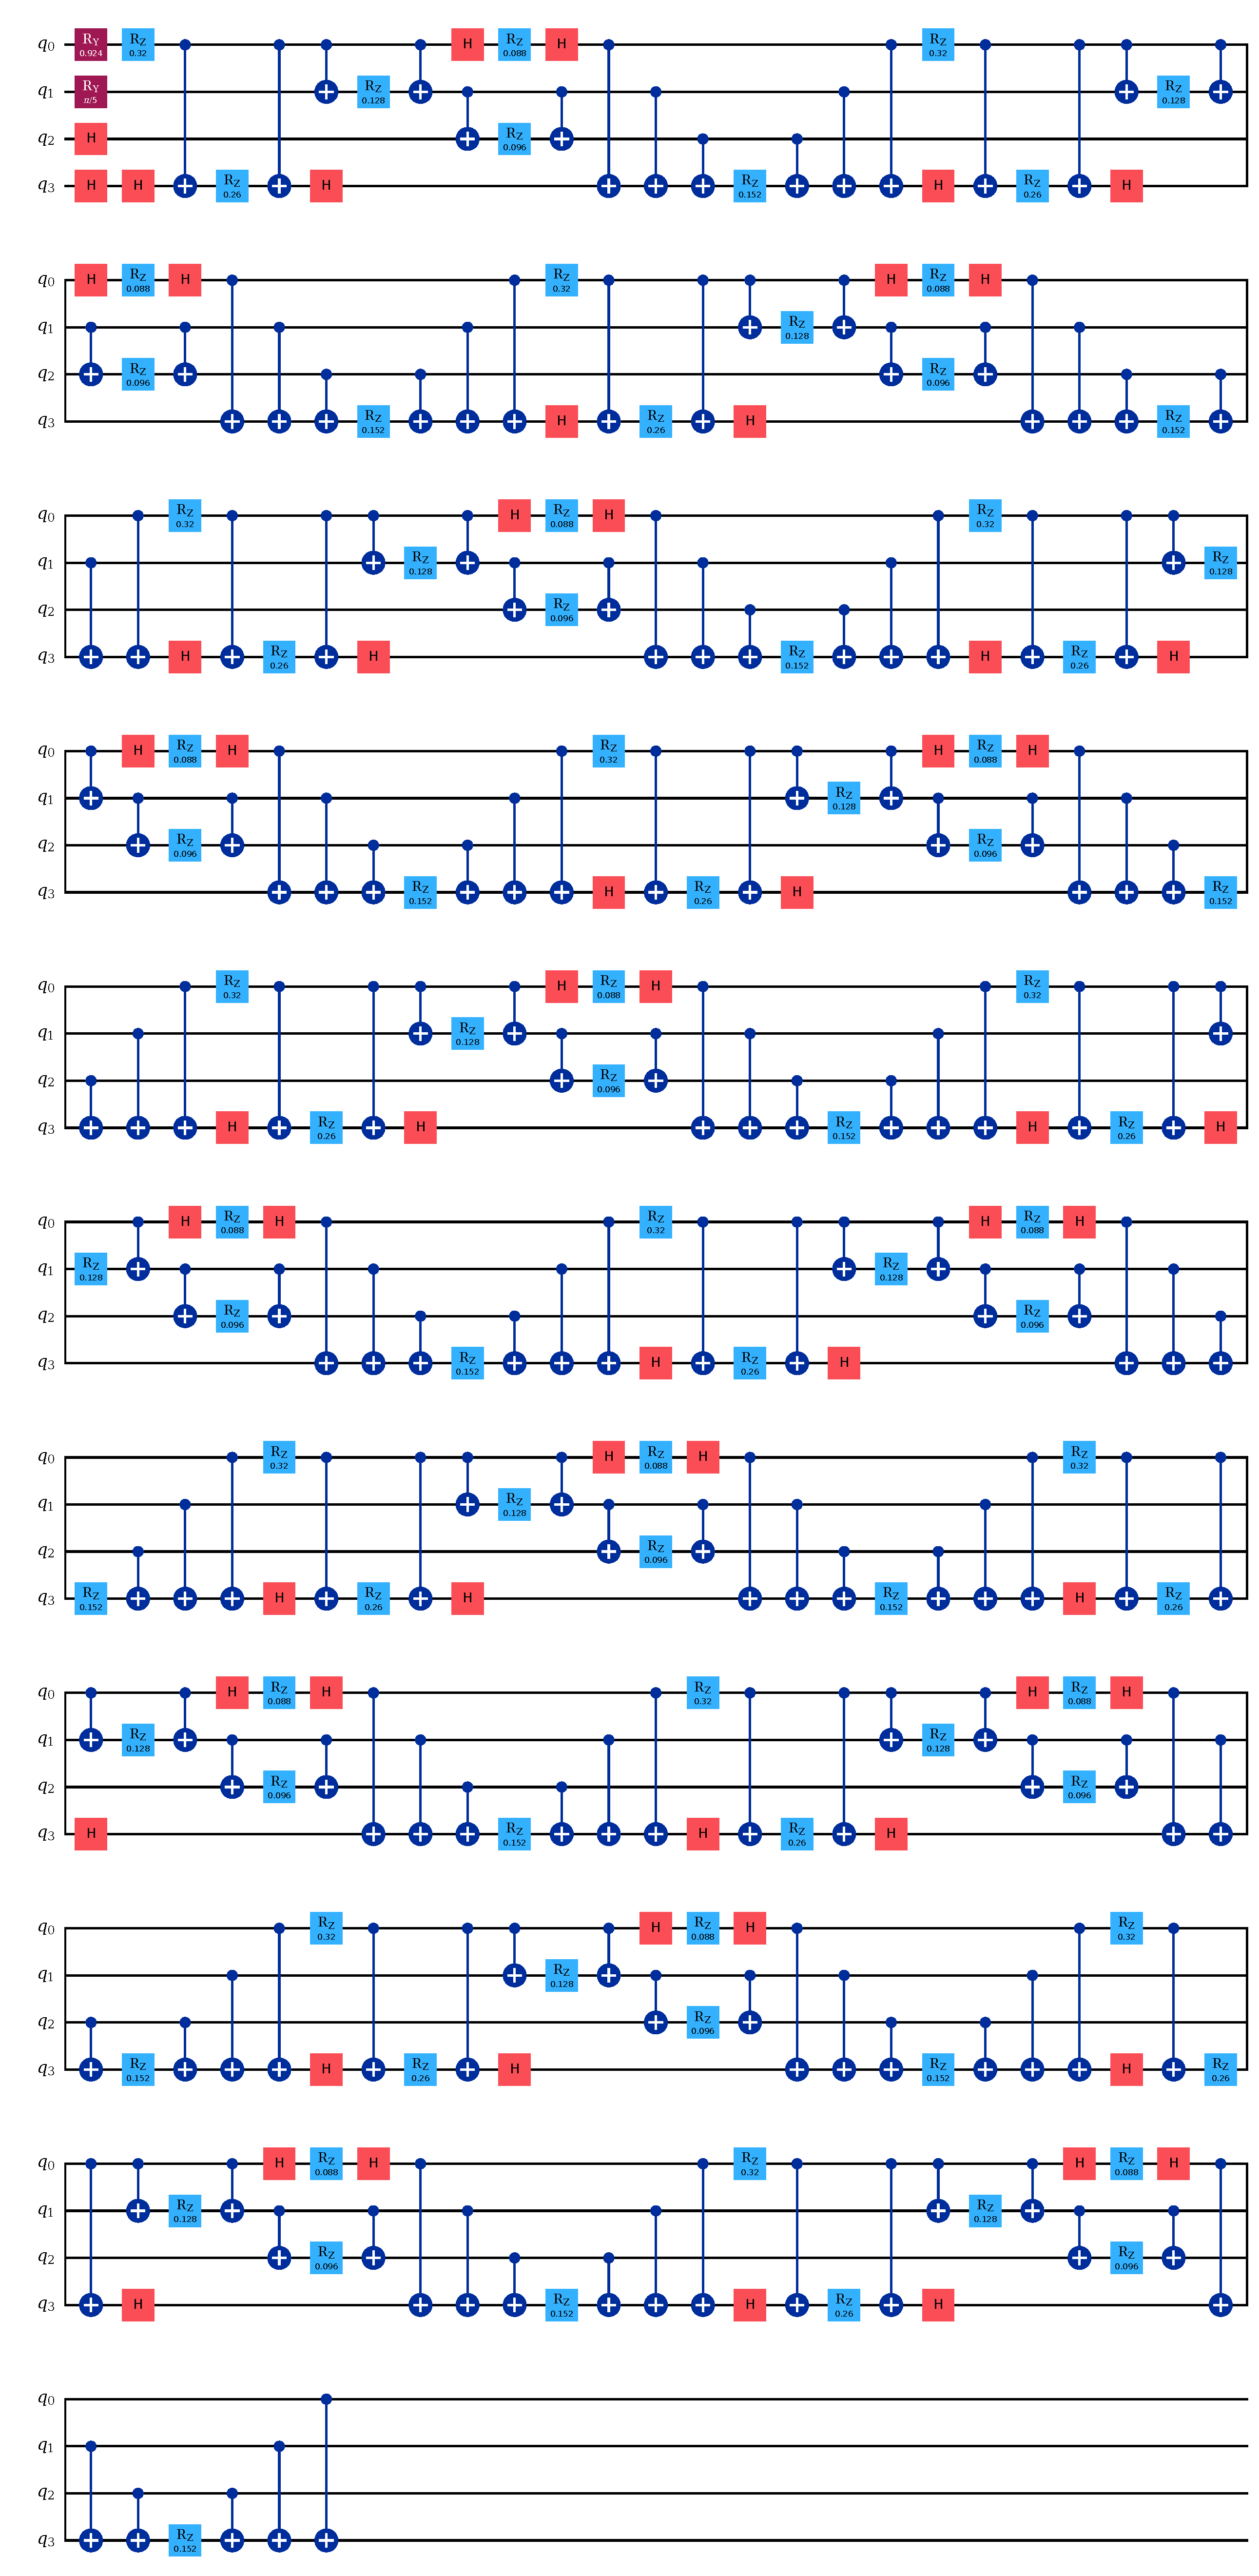
\includegraphics[width=0.52\textwidth]{demo_edt_gyro_trotter_4q_circuit_example.pdf}
\caption{\textbf{S7 | 4-qubit plaquette Trotter realization of EDT dynamics.}
Representative first-order Trotter circuit for an archived plaquette-style four-qubit workflow. The plaquette unitary $e^{-i \lambda Z_0 Z_1 Z_2 Z_3}$ generates multi-qubit entanglement associated with loop topology, while the remaining gates illustrate the inclusion of local control and interaction terms in a gate-based implementation.}
\label{fig:si_4q_plaquette_trotter_circuits}
\end{figure*}


\section{Noise and Robustness Checks}

Time evolution under the minimal plaquette Hamiltonian is approximated using first-order Trotterization, with circuit depth and gate count scaling linearly with evolution time~\cite{Trotter1959,Suzuki1990,Lloyd1996,Childs2019}. Observable errors are quantified by comparing exact and Trotterized expectation values~\cite{BerryAhokasCleveSanders2007}. The archived circuit figure in Sec.~S7 should therefore be interpreted as an implementation template for plaquette-style dynamics rather than as the only possible decomposition of the stripped-down Hamiltonian used in the main-text lambda sweep.

The finite dynamical regime is characterized by sweeping the loop strength $\lambda$ and identifying the optimal value $\lambda^\star$ that maximizes $S_{\mathrm{dyn}}$. Robustness in the present manuscript is evaluated in two ways: by repeating the exact sweep for several transverse-field values $h$ and several fixed $J$ values, and by comparing exact and Trotterized evolutions to verify that the finite optimum remains meaningful under approximate implementation~\cite{Childs2019}.


\section{NV XY8 Model}

Quantum sensing in NV-center ensembles is analyzed within a quantum resource engineering framework using a rate-based model (\texttt{nvratemodel} API)~\cite{NVRateModel2023,Degen2017,Barry2020}. For XY8 dynamical-decoupling sequences, the control parameter set is defined as
\begin{equation}
\mathcal{C} = \{P_{\mathrm{laser}},\, t_{\mathrm{read}},\, \Omega_{\mathrm{MW}},\, \tau,\, N_{\pi},\, B_0,\, T,\, \mathrm{strain}\},
\end{equation}
which determines initialization, control, and environmental conditions of the sensor~\cite{Casola2018}.

These controls are mapped onto an effective resource vector
\begin{equation}
\mathcal{R} = \{R_{\mathrm{ph}},\, C,\, T_2(N_{\pi}),\, \chi(\omega),\, \mathrm{duty}\},
\end{equation}
where $R_{\mathrm{ph}}$ is the detected photon rate, $C$ is the fluorescence contrast, $T_2(N_{\pi})$ is the coherence time under dynamical decoupling, $\chi(\omega)$ is the filter-function response, and $\mathrm{duty}$ accounts for initialization and readout overhead. The filter function is peaked near $\omega \simeq \pi/\tau$, enabling frequency-selective amplification of ac fields~\cite{Cywinski2008}.

Sensing performance is quantified by a sensitivity proxy $\eta_{\mathrm{AC}}(\omega)$, which scales approximately as
\begin{equation}
\eta_{\mathrm{AC}}(\omega) \propto \frac{1}{\chi(\omega)\,C\,\sqrt{R_{\mathrm{ph}}\,T_2(N_{\pi})}} \times f_{\mathrm{duty}},
\end{equation}
consistent with standard analyses of NV magnetometry sensitivity~\cite{Degen2017,Barry2020}. Parameter sweeps over $(\tau,N_{\pi})$ identify optimal sensing configurations and reveal a finite optimum set by the competition between filter gain, coherence, pulse errors, and timing overhead~\cite{Cywinski2008,Casola2018}.


\section{Reproducibility}

The reproducibility assets for this manuscript are organized in the repository root. The directory \texttt{scripts/} contains figure-generation and analysis code, \texttt{data/} contains bundled data products used by the companion workflows, \texttt{tests/} contains automated checks for the packaged Python modules, and \texttt{figures/} contains the PRX-style main and supplementary figure assets copied from the legacy manuscript workspace.

For the K$_3$C$_{60}$ case study, the main reproducibility entry point is \texttt{scripts/make\_fig2\_k3c60\_edt.py}. Running \texttt{python scripts/make\_fig2\_k3c60\_edt.py} regenerates the curvature panels used in the main-text K$_3$C$_{60}$ figure, the supplementary robustness figure \texttt{figures/supplementary/S5\_threshold\_bootstrap.pdf}, and the summary file \texttt{data/k3c60/k3c60\_edt\_window\_summary.json} from the bundled curvature export \texttt{data/k3c60/tmp.agr}.

For the cross-material controls, the main reproducibility entry point is \texttt{scripts/make\_figS4\_material\_controls.py}. Running \texttt{python scripts/make\_figS4\_material\_controls.py} regenerates the supplementary comparison figure \texttt{figures/supplementary/S4\_material\_controls.pdf} and the processed summary table \texttt{data/processed/material\_controls\_summary.csv} from the archived curvature exports in \texttt{data/na/}, \texttt{data/v/}, \texttt{data/lah10/}, and \texttt{data/ybacu3o7/}, together with the K$_3$C$_{60}$ reference export.

For the plaquette-dynamics case study, the main reproducibility entry point is \texttt{scripts/fig4\_plaquette\_dynamics.py}. Running \texttt{python scripts/fig4\_plaquette\_dynamics.py} regenerates the main-text dynamics figure \texttt{figures/main/fig4\_plaquette\_dynamics.pdf} and the processed sweep table \texttt{data/processed/plaquette\_lambda\_sweep.csv}. The stripped-down model implementation used by that script is the package \texttt{src/plaquette\_model}.

Across all systems studied, curvature arising from electron--vibration interaction defines structured manifolds in which electronic states are organized and degeneracies are lifted. This establishes curvature as the microscopic origin of EDT and links the manuscript claims to specific analysis scripts and figure products in the repository.


\bibliography{references}

\end{document}

